\documentclass{write_paper} 
\usepackage{amsmath}
\usepackage{ctex}
\usepackage{url}
%\usepackage{algorithm}
\usepackage{booktabs}
\usepackage{multirow}
\usepackage{algpseudocode}
\usepackage{subfigure}
\usepackage{epsfig}
\usepackage[utf8]{inputenc}
\usepackage[linesnumbered, ruled, vlined]{algorithm2e}
\usepackage{amsmath}
\usepackage{booktabs}
\usepackage{multirow}
\usepackage{wrapfig}  % 确保导言区引入该包
\usepackage{tikz}
\usepackage{fontspec}
\usetikzlibrary{positioning, arrows.meta}
\usepackage{caption}
\setmainfont{Segoe UI Emoji}  % Windows 推荐
% \setmainfont{Noto Color Emoji}  % Linux 推荐

 
\usepackage{siunitx}
  
\sisetup{group-separator={,}} % 千位分隔符


\usepackage[hidelinks]{hyperref}
\hypersetup{
  colorlinks=true,
  linkcolor=blue,
  filecolor=magenta,      
  urlcolor=blue,
  citecolor=blue,
}
\makeatletter
\@ifundefined{newblock}{\def\newblock{\hskip .11em plus .33em minus .07em}}{}
\makeatother

\usepackage{enumitem}
\makeatletter
\renewcommand\section{\@startsection {section}{1}{\z@}%
                                   {-1ex \@plus -1ex \@minus -.1ex}%
                                   {1 ex \@plus.1ex}%
                                   {\normalfont\large\bfseries}}
\renewcommand\subsection{\@startsection{subsection}{2}{\z@}%
                                     {-1ex\@plus -1ex \@minus -.1ex}%
                                     {1ex \@plus .1ex}%
                                     {\normalfont \normalsize \bfseries}}
\renewcommand\subsubsection{\@startsection{subsubsection}{3}{\z@}%
                                     {-1ex\@plus -1ex \@minus -.1ex}%
                                     {1ex \@plus .1ex}%
                                     {\normalfont\normalsize\bfseries}}
\makeatother

\renewcommand{\theARTICLETOP}{}
\usepackage{fancyhdr}
\pagestyle{fancy}
\fancyhf{}
\fancyhead[LE,RO]{}
\fancyhead[RE,LO]{\scriptsize{计算金融与仿真课程论文} }
\fancyfoot[CE,CO]{\leftmark}
\cfoot{\thepage}

\usepackage[T1]{fontenc}
\usepackage{palatino}

\OneAndAHalfSpacedXI
\usepackage{color}
\usepackage{soul}

\DeclareMathOperator{\E}{\mathbb{E}}
\DeclareMathOperator{\R}{\mathbb{R}}
\DeclareMathOperator{\B}{\mathbb{B}}
\DeclareMathOperator{\Z}{\mathbb{Z}}

%%-----------------------------------------
%% 将作者-年份改为数字制
\usepackage[numbers]{natbib}  % 关键:numbers选项
% \bibpunct{[}{]}{,}{n}{}{,}   % 若需要可自行指定标点
%%-----------------------------------------

% 如果之前有 \bibpunct 设置, 请注释掉或删除以免冲突
% \bibpunct[, ]{(}{)}{,}{a}{}{,}%  <-- 原先作者-年份制, 需要注释或删除

\TheoremsNumberedThrough
\EquationsNumberedThrough
\MANUSCRIPTNO{} 
\newtheorem{prop}{{Proposition}}
%\newtheorem{lemma}{{Lemma}}

%\renewcommand{\algorithmicrequire}{{Input:}}
%\renewcommand{\algorithmicensure}{{Output:}}

\newtheorem{implication}{\noindent{Implication}}

\newcommand{\YH}[1]{{\color{blue}#1}}
\newcommand{\JJ}[1]{{\color{black}#1}}
\newcommand{\eat}[1]{}
\usepackage{graphicx}
\usepackage{listings}
\usepackage{xcolor}  % 可选:定义颜色

\lstset{
  language=Python,             % 设置语言
  basicstyle=\ttfamily\tiny, % 基本字体风格
  numbers=left,               % 行号位置,可选 right 或 none
  numberstyle=\tiny,          % 行号字体
  keywordstyle=\color{blue},  % 关键字颜色
  commentstyle=\color{gray},  % 注释颜色
  stringstyle=\color{orange}, % 字符串颜色
  backgroundcolor=\color{white}, % 背景色
  frame=single,               % 添加边框,可选 shadowbox/double
  breaklines=true,            % 自动换行
  captionpos=b,               % 标题位置,b 或 t
  tabsize=4,                  % tab 宽度
  showstringspaces=false,     % 不显示字符串中的空格
}

\usepackage{endnotes}
\let\footnote=\endnote
\def\notesname{Endnotes}

\usepackage[symbol]{footmisc}
\renewcommand{\thefootnote}{\fnsymbol{footnote}}

\newcommand{\bs}[1]{\boldsymbol{#1}}
\newcommand{\ml}[1]{\mathcal{#1}}
\newcommand{\mb}[1]{\mathbb{#1}}

\begin{document}

% 整页垂直居中
\vspace*{\fill}

\begin{center}

    
\includegraphics[width=0.4\textwidth]{Figures/校徽.png}\\[1cm]
       \Huge \bfseries
      {计算金融与仿真}\\[0.5cm]
       \Huge \bfseries
      {课程论文}\\[2cm]
    
    \Large
    \begin{table}[htbp]
    \centering
    \Large
    \begin{tabular}{ll}
   {论文题目 }: & 计算金融与仿真 \\
   {学生姓名}: & 李晶晶 \quad 张璐 \quad 朱冯婧 \\
   {指导老师}: & 邓智斌 
    \end{tabular}
    \end{table}

    


\end{center}

\vspace*{\fill}
\newpage
 



\section{投资组合选择介绍}

P2P 借贷(Peer-to-Peer Lending)是一种通过互联网平台撮合借贷双方、绕过传统金融机构中介的融资方式。该模式简化了借贷流程,降低了交易成本,使借款人能以相对较低利率获得融资,同时也为投资者提供了相较于银行存款或债券更高的潜在收益。投资者可将资金分散投入至多个借款人,借助平台风险评级体系控制整体违约风险。

当前,全球主流的 P2P 平台包括 LendingClub、Prosper、Funding Circle 等,其中 LendingClub 是美国最大且最具代表性的 P2P 借贷平台之一。平台通常依据借款人的 FICO 分数、贷款金额与期限、债务状况、收入水平、就业类型等信息为贷款项目分配信用等级,并据此帮助投资者评估其风险与回报潜力。本文选取 LendingClub 的公开数据(涵盖 2007--2018 年贷款记录),并基于借款属性推算违约概率,用于后续建模与优化分析。

从决策角度看,投资者在贷款配置时不仅关注收益水平,还需兼顾风险控制与资金约束。在资金有限的情况下,如何从大量贷款项目中选择最优子集、构建风险可控的投资组合,是一个典型的组合优化问题。与传统证券类投资组合优化不同,P2P 投资需处理的风险变量更为复杂,需结合借款人层面的个体信用风险评估。

大量学者针对 P2P 投资组合决策开展了研究。Wan 等人~\cite{wan2023hybrid} 通过引入混合治愈模型(Mixture Cure Model, MCM)刻画借款人违约行为,并将投资者目标建模为收益最大与风险最小的双目标优化问题。Guo 等人~\cite{guo2016instance} 基于 LendingClub 和 Prosper 数据集,提出实例驱动的风险评估方法,从风险最小化角度出发构建组合优化模型。Byanjankar 等人~\cite{byanjankar2021data} 将该问题建模为多目标最优化任务,并在相似性计算中融合核方法与期望框架,取得优于传统方法的效果。

在风险量化工具方面,金融领域广泛采用 VaR(Value at Risk)和 CVaR(Conditional Value at Risk)作为核心指标。VaR 表示在置信水平 $\alpha$ 下,未来特定时间窗口内最大可能损失;CVaR 则进一步衡量超过 VaR 值的极端尾部损失的期望值,是更为保守和稳健的风险度量方式。与 VaR 相比,CVaR 可更好地识别低概率高损失事件,在风险厌恶型投资组合设计中具有广泛应用价值。

值得注意的是,尽管 P2P 借贷在国外仍保持活跃,但在中国的发展路径经历了兴盛与衰退的剧烈波动。2013--2017 年间,中国 P2P 平台数量激增,借贷余额快速攀升,成为普惠金融的重要支撑力量。然而,由于监管滞后、信用审核不足与资金池乱象等问题频发,平台跑路、“爆雷”等现象不断,严重影响投资者信心。自 2018 年起,中国政府开始全面整顿该行业,2020 年中国银保监会正式宣布“P2P 网贷机构全部清零”,宣告传统意义上的 P2P 模式在中国全面退出。

尽管如此,P2P 模式所蕴含的“去中介化”融资理念、分散化投资逻辑与风险共担机制,依然对当下诸如数字信贷、消费金融、场景金融等新兴平台具有重要借鉴意义。例如,微粒贷、借呗、360 借条等互联网信贷产品实质上仍在匹配海量个人借贷需求与分布式资金供给。借助更完善的风控系统与信息披露机制,这些平台正延续并演进着 P2P 的基本逻辑。

因此,在“后 P2P 时代”,围绕借款人信用特征建模、投资组合风险控制与收益优化的问题仍具有显著的现实意义与研究价值。本文基于 LendingClub 数据集,从贷款违约概率出发构建收益函数,并引入 VaR/CVaR 等风险约束,设计组合优化模型,结合粒子群算法与整数规划工具协同求解,旨在为现实场景下投资者如何在风险可控前提下进行有效资金配置提供理论支持与方法参考。

 
\section{模型建立}

在贷款投资组合优化问题中,投资者需在收益与风险之间寻求平衡,而传统的期望收益最大化模型往往无法充分刻画潜在损失的不确定性。为更科学地反映风险偏好并提升模型的现实适应性,本文引入多种风险控制机制,构建一套逐步递进的优化模型体系。首先,需要明确所采用的风险度量方法,以作为后续模型设计的基础。

\subsection{风险度量方法概述:VaR 与 CVaR}

在实际投资决策中,单纯追求期望收益往往难以充分反映投资组合所面临的潜在风险,尤其在 P2P 贷款等高风险资产配置场景中,损失的不确定性更不容忽视。投资者更倾向于关注极端情形下的损失程度及其发生概率,因此,在构建优化模型时引入科学有效的风险度量方法尤为关键。本文选取两种在金融风险管理领域中广泛应用的风险度量工具,即风险价值VaR与条件风险价值CVaR,作为模型设计的基础。

\paragraph{VaR} 用于衡量在给定置信水平 $\beta$ 下,投资组合在未来某一持有期内可能遭受的最大损失。设组合损失为随机变量 $L$,其数学定义为:
\[
\text{VaR}_\beta(L) = \inf \left\{ \eta \in \mathbb{R} \mid \mathbb{P}(L \leq \eta) \geq \beta \right\},
\]
即在置信水平 $\beta$ 下,损失超过 $\text{VaR}_\beta$ 的概率不超过 $1 - \beta$。VaR 能较好地描述常规市场波动下的最大潜在损失,但在捕捉尾部风险方面存在局限。

\paragraph{CVaR} 在 VaR 的基础上进一步引入对尾部损失的刻画,其定义为在损失超过 VaR 水平的条件下的期望损失:
\[
\text{CVaR}_\beta(L) = \mathbb{E}[L \mid L \geq \text{VaR}_\beta(L)].
\]
CVaR 能更全面地反映极端情况下的平均损失程度,是一种更为稳健的风险控制工具,尤其适用于高度风险厌恶型的投资者。在优化建模中,CVaR 通常被认为比 VaR 更具保守性和可解释性。
\subsection{模型设定与参数说明}

为系统性地构建贷款投资组合优化问题,本文首先明确模型所涉及的核心参数,如表~\ref{tab:parameters} 所示。该参数体系涵盖贷款项目的基本属性、投资者的预算限制、风险容忍度约束以及信用等级的分散配置要求,构成后续优化建模与求解的基础。

\begin{table}[htbp]
\centering
\caption{模型参数说明}
\label{tab:parameters}
\begin{tabular}{ll}
\toprule
符号 & 含义 \\
\midrule
$x_i$ & 决策变量,若选择第 $i$ 个贷款项目则 $x_i = 1$,否则为 $0$ \\
$A_i$ & 第 $i$ 个贷款的申请金额 \\
$r_i$ & 第 $i$ 个贷款的年利率 \\
$P_i$ & 第 $i$ 个贷款的违约概率 \\
$B$ & 投资者可用于配置的总预算 \\
$R_{\max}$ & 可接受的最大预期违约损失 \\
$G_k$ & 信用等级类别 $k$ 所对应的贷款集合 \\
$\alpha_k$ & 信用等级 $k$ 对应的投资金额占比上限 \\
$m$ & 可选贷款项目数量的上限(Top-$m$) \\
\bottomrule
\end{tabular}
\end{table}

\subsection{模型构建}

在前述参数设定基础上,本文构建一类面向贷款投资组合优化的数学模型族,以适应不同风险偏好下的投资策略制定。首先定义可行解集合 $\mathcal{X}$,即所有满足投资者约束条件的贷款选择方案:
\[
\mathcal{X} = 
\left\{ x=(x_1,\cdots,x_N) \in \{0,1\}^N \;\middle|\;
\begin{aligned}
  &\sum_{i=1}^N x_i \leq m, \\
  &\sum_{i=1}^N x_i A_i \leq B, \\
  &\sum_{i \in G_k} x_i A_i \leq \alpha_k B,\quad \forall k 
\end{aligned}
\right\},
\]
其中,$N$ 表示可选贷款项目的总数,$x_i$ 为第 $i$ 个项目的选择变量。

基于该可行域,本文依次构建三个层次递进的优化模型,分别聚焦于期望回报最大化、极端损失控制与尾部风险抑制,以覆盖从风险中性到高度风险规避的不同投资情境。

首先构建基础模型,以最大化贷款组合的期望回款为目标。在控制预算、信用等级配置及总违约损失的前提下,优化组合的平均收益水平:
\begin{equation}
\begin{aligned}
\max_{x\in\mathcal{X}} \quad & \sum_{i=1}^N x_i A_i r_i(1 - P_i) \\
\text{s.t.} \quad & \sum_{i=1}^N x_i A_i P_i \le R_{\max},
\end{aligned}
\label{eq:main_model}
\tag{P2P}
\end{equation}

为了控制极端情境下的损失概率,引入基于 VaR 的风险约束机制。该模型通过场景模拟,限制超出损失阈值 $\eta$ 的场景数量不超过置信水平对应的容忍范围 $(1 - \beta)S$:
\begin{equation}
\begin{aligned}
\max_{x\in\mathcal{X},z_s} \quad & \sum_{i=1}^N x_i A_i r_i(1 - P_i) \\
\text{s.t.} \quad
& \sum_{i=1}^N x_i A_i \cdot \tilde{P}_i^{(s)} - \eta \le \mathcal{M} z_s, \quad \forall s = 1,\dots,S, \\
& \sum_{s=1}^S z_s \le (1 - \beta) S, \\
& z_s \in \{0,1\}, \quad \forall s = 1,\dots,S,
\end{aligned}
\label{eq:var_model}
\tag{P2P-VaR}
\end{equation}
其中,$\tilde{P}_i^{(s)}$ 表示情景 $s$ 下第 $i$ 个贷款项目的违约概率估计,$z_s$ 为辅助二进制变量,$\mathcal{M}$ 为足够大的惩罚常数。

在此基础上进一步考虑尾部损失的严重程度,构建包含 CVaR 限制的稳健模型。该模型在控制损失超过 VaR 的概率基础上,进一步限制这些超额损失的期望值不超过预设上限 $\text{CVaR}_{\max}$:
\begin{equation}
\begin{aligned}
\max_{x\in\mathcal{X},\xi_s} \quad & \sum_{i=1}^N x_i A_i r_i(1 - P_i) \\
\text{s.t.} \quad
& \xi_s \ge \sum_{i=1}^N x_i A_i \cdot \tilde{P}_i^{(s)} - \eta, \quad \forall s = 1,\dots,S, \\
& \eta + \frac{1}{S(1 - \beta)} \sum_{s=1}^S \xi_s \le \text{CVaR}_{\max}, \\
& \xi_s \ge 0, \quad \forall s = 1,\dots,S,
\end{aligned}
\label{eq:cvar_model}
\tag{P2P-CVaR}
\end{equation}
其中,$\xi_s$ 表示每个情景中损失超出 VaR 水平的超额部分,CVaR 约束通过平均化尾部损失,提升组合对极端风险的适应性。

综上,模型~\eqref{eq:main_model} 适用于追求平均收益、风险承受能力较强的投资者;模型~\eqref{eq:var_model} 通过 VaR 控制极端损失的概率,适用于稳健投资偏好者;模型~\eqref{eq:cvar_model} 则在此基础上进一步引入 CVaR 限制,更适合风险厌恶型投资者。该三层次模型体系为贷款投资组合提供了灵活且可调的策略选择框架。
\section{算法设计}

在贷款投资组合优化问题中,面临着非线性、非凸性与整数变量约束等多重挑战,传统优化方法往往难以在合理时间内获得高质量解。为此,本文引入粒子群优化算法(Particle Swarm Optimization, PSO)与 Gurobi 求解器相结合的两阶段优化框架,旨在兼顾全局搜索能力与精确求解能力,提升模型在大规模金融数据环境下的求解效率与稳健性。该联合方法通过 PSO 快速获取近优可行解,再利用 Gurobi 进行高精度强化求解,为解决具有复杂约束结构的信贷资源配置问题提供了一种有效的技术路径。

\subsection{粒子群优化算法(PSO)}

粒子群优化算法(Particle Swarm Optimization, PSO)是一种基于群体智能的随机优化方法,由 Kennedy 和 Eberhart 于 1995 年首次提出~\cite{kennedy1995particle}。该算法受鸟群觅食行为的启发,模拟粒子在解空间中基于个体经验与群体经验协同搜索最优解的过程,具备良好的全局搜索能力和并行性。

在 PSO 中,每个粒子表示一个潜在解,其状态由位置向量和速度向量构成。粒子在每一代的搜索过程中,根据其个体历史最优位置(Personal Best, $pbest$)与群体历史最优位置(Global Best, $gbest$)共同引导其飞行方向和速度调整。更新公式如下所示:
\[
\begin{aligned}
v_i^{(t+1)} &= w \cdot v_i^{(t)} + c_1 \cdot r_1 \cdot (pbest_i - x_i^{(t)}) + c_2 \cdot r_2 \cdot (gbest - x_i^{(t)}), \\
x_i^{(t+1)} &= x_i^{(t)} + v_i^{(t+1)},
\end{aligned}
\]
其中,$x_i^{(t)}$ 和 $v_i^{(t)}$ 分别表示第 $i$ 个粒子在第 $t$ 代的位置信息与速度;$w$ 是惯性权重,用于平衡全局搜索与局部开发能力;$c_1$ 和 $c_2$ 分别为个体学习因子与社会学习因子;$r_1, r_2 \sim U(0,1)$ 是均匀分布的随机数,引入搜索的随机扰动。

PSO 算法具有实现简单、参数调节较少、搜索效率高等优点,尤其适用于复杂非凸、不可导甚至离散的组合优化问题。然而,其缺点在于缺乏全局最优性保证,容易陷入局部最优,故常用于快速生成高质量初始解或作为启发式模块与精确优化方法联合使用。

\subsection{PSO 与 Gurobi 的联合优化框架}

\begin{wrapfigure}{l}{0.45\textwidth}
\vspace{-1ex}
\centering
\begin{tikzpicture}[node distance=1.5cm, every node/.style={font=\small}]
  \tikzstyle{startstop} = [rectangle, rounded corners, minimum width=4cm, minimum height=0.8cm, text centered, draw=black, fill=blue!10]
  \tikzstyle{process} = [rectangle, minimum width=4cm, minimum height=0.8cm, text centered, draw=black, fill=gray!10]
  \tikzstyle{arrow} = [thick,->,>=stealth]

  \node (start) [startstop] {初始化参数};
  \node (pso) [process, below of=start] {PSO 粒子群搜索};
  \node (decode) [process, below of=pso] {解码粒子位置};
  \node (select) [process, below of=decode] {选取最优候选解};
  \node (gurobi) [process, below of=select] {Gurobi 精确求解};
  \node (end) [startstop, below of=gurobi] {输出最优结果};

  \draw [arrow] (start) -- (pso);
  \draw [arrow] (pso) -- (decode);
  \draw [arrow] (decode) -- (select);
  \draw [arrow] (select) -- (gurobi);
  \draw [arrow] (gurobi) -- (end);
\end{tikzpicture}
\caption{PSO 与 Gurobi 联合优化框架}
\label{fig:framework}
\vspace{-1ex}
\end{wrapfigure}

为兼顾搜索效率与解的精度,本文提出了一种融合粒子群优化(PSO)与整数规划求解器 Gurobi 的两阶段联合优化框架,如图~\ref{fig:framework} 所示。该框架充分发挥了 PSO 在大规模组合优化中的全局搜索能力,同时利用 Gurobi 在整数规划领域的精确性,显著提升了最终解的质量与可行性。

第一阶段为启发式搜索阶段,PSO 用于在高维、复杂约束的可行域中高效生成优质解。粒子的连续位置向量经特定解码机制转换为 0-1 决策向量,并据此评估目标值与约束可行性。在多轮迭代演化后,选取适应度最优的粒子解作为候选输入。

第二阶段为精确优化阶段,将 PSO 输出的最优候选解作为 warm-start 初始化输入至 Gurobi,构建并求解相应的混合整数规划模型,以获得满足所有约束的最优或近似最优解。

为进一步提升求解效率与模型稳健性,本文设计了如下机制:
\begin{itemize}
    \item 设计连续到二进制的粒子位置解码规则,确保每一粒子解在语义上合法;
    \item 引入精英保留机制,避免 Gurobi 从劣质粒子解出发,缩短求解时间;
    \item 在 PSO 阶段主动筛除不满足基本约束的无效粒子,降低冗余计算;
    \item 设置 Gurobi 最大运行时间与 MIPGap 阈值,权衡解质量与计算开销。
\end{itemize}

从复杂度角度来看,该问题属于典型 NP-难问题,Gurobi 求解整数规划模型的最坏时间复杂度为指数级;PSO 每轮迭代的计算复杂度为 $\mathcal{O}(n \cdot d)$,其中 $n$ 为粒子数,$d$ 为变量维度。尽管缺乏全局最优性保证,该联合优化框架在实证测试中展现出良好的收敛速度与求解效果。

综上所述,PSO + Gurobi 联合优化框架通过“粗定位 + 精求解”的两阶段策略,实现了群体智能与数学规划的优势互补,特别适用于结构复杂、变量众多的贷款投资组合优化问题,具有较高的计算效率与工程适用性。

\section{案例研究}
\label{sec:case_study}

为验证所提出模型在实际场景下的有效性,本文基于真实平台数据开展实证分析,依次介绍数据集来源与处理方式、违约概率预测模型的训练方法、三类优化模型的构建与求解流程,并对比评估不同模型的优化效果。

\subsection{数据集描述}

\label{subsec:dataset_description}

本研究使用的数据集来自 Lending Club 平台, 原始数据由 Kaggle 网站\url{https://www.kaggle.com/datasets/wordsforthewise/lending-club}公开提供. Lending Club 是美国最大的网络借贷平台之一, 提供了详尽的个人借款申请及其还款情况的数据, 广泛应用于学术界和工业界进行信贷风险评估, 违约预测及投资组合优化等研究. 

该数据集包含了从 2007 年至 2018 年的借款记录, 共计数百万条样本. 每条记录对应一笔贷款申请, 涵盖了包括贷款金额, 利率, 借款人信用等级, 债务收入比, 贷款期限, 还款状态, 就业年限, 收入, 地址状态, 房屋所有权, FICO 评分区间等在内的多维度信息. 

在本研究中, 我们主要筛选并保留11种变量用于建模分析,如表\ref{tab:dataset_variables}所示. 这些变量涵盖了借款人的基本信息, 贷款合同的核心条款以及还款状态等关键信息, 为后续的风险评估与投资组合优化提供了必要的数据基础.
\begin{table}[htbp]
\centering
\caption{建模所用主要变量说明}
\label{tab:dataset_variables}
\begin{tabular}{ll}
\toprule
变量名称 & 含义说明 \\
\midrule
\texttt{loan\_amnt} & 借款人申请的贷款金额,对应模型中的 $A_i$ \\
\texttt{int\_rate} & 借款合同中约定的年利率,用于计算收益率 $r_i$ \\
\texttt{grade} & 借款人信用等级(A 至 G),用于构建信用等级集合 $G_k$ \\
\texttt{loan\_status} & 实际贷款还款状态(如 Fully Paid, Charged Off),用于推断违约情况 \\
\texttt{annual\_inc} & 借款人年收入,用于辅助风险刻画 \\
\texttt{dti} & 债务收入比(Debt-to-Income Ratio),用于增强风险特征描述 \\
\texttt{term} & 贷款期限(如 36 months 或 60 months) \\
\texttt{emp\_length} & 借款人工作年限 \\
\texttt{addr\_state} & 借款人所在州(美国各州) \\
\texttt{fico\_range\_high} & 借款人 FICO 信用评分上限,用于量化信用水平 \\
\texttt{fico\_range\_low} & 借款人 FICO 信用评分下限,用于量化信用水平 \\
\bottomrule
\end{tabular}
\end{table}
 

为了满足模型中对违约概率 $P_i$ 的需求, 使用机器学习预测违约概率作为后续优化模型的输入. 具体方法将在后续章节详细介绍.

此外, 为模拟贷款违约的风险场景, 我们以借款人的信用等级, FICO评分和历史违约频率为依据, 构建了 $S$ 个 Monte Carlo 风险场景, 用于后续 CVaR 优化模型的风险评估. 

通过上述数据处理步骤, 最终形成了一个结构规范, 信息完备, 适用于组合优化问题的数据集, 为后续实证分析与建模提供了坚实的数据基础. 

\begin{table}[htbp]
\centering
\caption{三类投资优化模型的主要参数设置}
\begin{tabular}{lll}
\toprule
 {参数符号} &{含义} &{适用模型} \\
\midrule
$B$ & 投资总预算,$1 \times 10^8$ 元 & 全部 \\
$m$ & 最多选择的贷款数量(Top-$m$),5000 & 全部 \\
$P_i$ & 贷款 $i$ 的违约概率,$P_i \in [0, 1]$ & 全部 \\
$R_{\max}$ & 风险容忍值上限,$1.5 \times 10^7$ 元 & 全部 \\
$\text{CVaR}_{\max}$ & 期望风险容忍值上限,$1.5 \times 10^7$ 元 & CVaR\\
$\beta$ & 置信水平(VaR、CVaR),0.95 & VaR ,CVaR\\
$\eta$ & VaR临界值(上界),动态变量 & VaR ,CVaR\\
$S$ & 蒙特卡洛模拟场景数量,1000 & VaR ,CVaR\\
$\alpha_k$ & 信用等级比例上限 & 全部\\
& \quad A: 40\%, B: 30\%, C: 20\%, D: 10\%, E: 5\%, F: 2\%, G: 1\% & \\
$pop\_size$ & 粒子群算法种群规模,30 & PSO  \\
$max\_iter$ & 粒子群最大迭代次数,100 & PSO  \\
$(w, c_1, c_2)$ & PSO 参数设置:$w=0.7$, $c_1=c_2=1.5$ & PSO  \\
\bottomrule
\end{tabular}
\label{tab:three-model-params}
\end{table}
\subsection{使用机器学习预测违约概率 $P_i$}
\label{subsec:predict_p_i}

尽管本研究使用的数据集中所有贷款均已获得实际资助, 但在资金有限, 需进行优选配置的情境下, 我们仍需要对这些已发放贷款的还款风险进行再评估. 为此, 我们引入机器学习方法, 对每笔贷款的未来违约概率 $P_i$ 进行预测建模, 以作为后续优化模型中的风险输入参数. 

 
预测函数的目标是:对于每笔已发放贷款 $i$, 根据其已知特征向量 $\mathbf{x}_i$, 估计其在未来发生违约的概率 $P_i = \mathbb{P}(y_i = 1 \mid \mathbf{x}_i)$. 其中, $y_i=1$ 表示贷款最终发生违约(如状态为 \texttt{Charged Off}), $y_i=0$ 表示贷款最终还清(如状态为 \texttt{Fully Paid}). 


我们基于借款人基本属性, 贷款合同信息以及信用评级等信息构建预测特征集, 涵盖表~\ref{tab:dataset_variables} 中列出的变量。
考虑到目标变量仍是二元状态(违约 / 未违约), 我们采用监督学习的二分类方法进行建模. 尝试的模型包括逻辑回归(Logistic Regression), 随机森林(Random Forest), 梯度提升树(GBDT), 极端梯度提升(XGBoost)等. 
由于样本中违约样本占比相对较小, 我们在训练过程中采用类别加权, 欠采样等方式处理类别不平衡问题. 
我们将全部已发放贷款随机划分为训练集(70\%)与测试集(30\%), 使用交叉验证调优参数, 并基于测试集评估模型表现. 评价指标包括准确率(Accuracy), AUC 值(Area Under the ROC Curve), F1 分数等. 
最终, 我们选择 AUC 表现最优的模型用于对所有贷款样本生成违约概率预测值 $\hat{P}_i$, 作为后续优化模型中的输入. 
 
虽然原始数据中每笔贷款都已实际放款, 但我们的建模任务是为现实中的“再选择”提供依据. 即在预算受限, 资源不足时, 如何在这些真实已放款的贷款中优先挑选违约概率低, 预期收益高的子集, 构建一个更稳健的投资组合. 因此, $\hat{P}_i$ 的预测并非用于决定放款与否, 而是作为组合优化的“风险估计量”, 用于构建期望收益与 CVaR 等风险指标. 
\subsection{三类优化模型的构建与求解}
\label{subsec:model_solving}

为系统刻画贷款投资组合在收益最大化与风险控制之间的权衡关系,本文依托模型~\eqref{eq:main_model}--\eqref{eq:cvar_model},设计并实现三类优化算法,分别反映不同风险偏好下的投资策略。算法~\ref{alg:primal_model} 基于期望损失约束,在预算、投资人数及信用等级配置要求下,最大化贷款组合的期望回款,适用于风险容忍度较高的投资者。为提升模型对极端损失的控制能力,算法~\ref{alg:var_model} 引入 VaR 约束,利用模拟场景的分位损失限制组合的最大潜在损失。考虑到 VaR 仅提供损失临界值而无法反映尾部损失的严重程度,算法~\ref{alg:cvar_model} 进一步引入 CVaR 约束,对超出 VaR 水平的损失均值进行限制,从而增强模型的稳健性。三种模型由“均值约束”逐步过渡至“尾部风险控制”,为投资者在不同风险容忍水平下提供具有针对性的最优策略生成方案。

\begin{algorithm}[htbp]  \footnotesize
\caption{原始模型:最大化期望回款}
\label{alg:primal_model}
\KwIn{贷款数据集:$A_i$, $r_i$, $P_i$, $grade_i$}
\KwOut{最优组合 $x_i \in \{0,1\}$}

\textbf{步骤1:收益与结构约束计算} \\
计算每笔贷款的期望收益 $profit_i = A_i \cdot r_i \cdot (1 - P_i)$ \\
构造信用等级分类 $G_k$ 与对应占比限制 $\alpha_k$

\textbf{步骤2:约束参数设定} \\
总预算 $B$,投资项目数量上限 $m$,期望损失阈值 $R_{\max}$

\textbf{步骤3:建立优化模型} \\
以 $\sum_i x_i \cdot profit_i$ 为目标函数,施加以下约束:
\begin{itemize}
  \item 预算约束:$\sum_i x_i A_i \leq B$
  \item 等级限制:$\sum_{i \in G_k} x_i A_i \leq \alpha_k B$
  \item 风险控制:$\sum_i x_i A_i P_i \leq R_{\max}$
  \item 数量限制:$\sum_i x_i \leq m$
\end{itemize}

\textbf{步骤4:模型求解} \\
调用 Gurobi 优化器,输出最优解及相应投资收益与组合结构。
\end{algorithm}

\begin{algorithm}[htbp]  \footnotesize
\caption{VaR 模型:引入分位损失约束}
\label{alg:var_model}
\KwIn{贷款数据集:$A_i$, $r_i$, $P_i$, $grade_i$}
\KwOut{最优组合 $x_i \in \{0,1\}$,VaR 风险值 $\eta$}

\textbf{步骤1:场景生成与收益计算} \\
构造 $S$ 个 Bernoulli 分布违约场景 $L_{i,s} \sim \text{Bernoulli}(P_i)$,计算 $profit_i$

\textbf{步骤2:参数设定与 VaR 控制阈值} \\
预算 $B$,人数上限 $m$,置信水平 $\beta$,VaR 阈值上限 $\eta_{\max}$

\textbf{步骤3:粒子群优化(PSO)初筛} \\
采用粒子群优化算法进行初步变量筛选,目标函数为:
\[
\max\ \sum_i x_i profit_i - \text{惩罚项}
\]
满足以下约束:
\begin{itemize}
  \item 预算与投资人数约束
  \item 信用等级配置约束
  \item 分位损失不超过 $\eta_{\max}$
\end{itemize}

\textbf{步骤4:Gurobi 精确求解} \\
引入辅助变量 $z_s$ 线性化 VaR 约束:
\[
\sum_i x_i A_i L_{i,s} - \eta \leq M \cdot z_s,\quad \sum_s z_s \leq (1 - \beta) S
\]
以 PSO 解作为初始点,构建混合整数规划模型求解最优策略。
\end{algorithm}

\begin{algorithm}[htbp]  \footnotesize
\caption{CVaR 模型:尾部风险控制下的组合优化}
\label{alg:cvar_model}
\KwIn{贷款数据集:$A_i$, $r_i$, $P_i$, $grade_i$}
\KwOut{最优组合 $x_i \in \{0,1\}$,CVaR 风险值}

\textbf{步骤1:数据处理与场景模拟} \\
清洗数据,构造期望收益 $profit_i$ \\
模拟 $S$ 个违约情景 $L_{i,s} \sim \text{Bernoulli}(P_i)$

\textbf{步骤2:CVaR 控制参数设定} \\
设定预算 $B$、人数上限 $m$、置信水平 $\beta$、CVaR 上限 $R_{\max}$

\textbf{步骤3:粒子群优化初始化} \\
定义 $\ell_s = \sum_i x_i A_i L_{i,s}$,CVaR 表达为:
\[
\text{CVaR}_\beta = \eta + \frac{1}{(1-\beta)S} \sum_{s=1}^S \max(0, \ell_s - \eta)
\]
最大化 $\sum_i x_i profit_i$,同时满足 CVaR 约束。

\textbf{步骤4:Gurobi 建模求解} \\
定义变量 $x_i$、$\eta$ 与 $\xi_s$,构建混合整数模型:
\[
\xi_s \ge \sum_i x_i A_i L_{i,s} - \eta,\quad \eta + \frac{1}{(1 - \beta)S} \sum_s \xi_s \le R_{\max}
\]
以粒子群输出解为初始值,求解最终最优组合。
\end{algorithm}

\subsection{结果分析}
\label{subsec:result_analysis}

为系统比较三类优化模型在不同风险控制机制下的投资表现,表~\ref{tab:result-comparison} 汇总了期望回款、入选贷款数量、VaR 与 CVaR 指标等核心结果,并区分使用 Gurobi 与 PSO 方法的求解效果。可以观察到,模型~\ref{eq:main_model}(无风险约束)在 Gurobi 求解下实现了最高的期望收益(约为 759 万元),但未引入任何尾部损失控制;而模型~\ref{eq:var_model} 和模型~\ref{eq:cvar_model} 则分别通过 VaR 和 CVaR 限制对极端损失进行了显式约束,尽管收益水平略有下降,却显著降低了尾部风险的暴露程度,体现了风险控制机制对最优解结构的实质性影响。

\begin{table}[htbp]
\centering
\caption{不同优化模型下的结果比较}
\label{tab:result-comparison}
\begin{tabular}{llllSSS}
\toprule
模型类型 & 方法 & 选中人数 & 投资组合期望收益 & {VaR 上界} & {CVaR 上界} \\
\midrule
\ref{eq:main_model}& Gurobi & 5000 & \textcolor{red}{\sisetup{group-separator={,}}\num{7596540.84}} & {--} & {--} \\
\midrule
\ref{eq:var_model}& PSO & 5000 & \num{7016573.73} & \num{36698075.00} & {--} \\
& Gurobi & 4157 & \textcolor{red}{\num{4803258.84}} & \num{16507725.00} & {--} \\
\midrule
\ref{eq:cvar_model} & PSO & 5000 & \num{7016573.73} & {--} & \num{36698075.00} \\
& Gurobi & 4347 & \textcolor{red}{\num{4774801.27}} & {--} & \num{14997692.00} \\
\bottomrule
\end{tabular}
\end{table}

图~\ref{fig:combined_results} 展示了三类模型所选贷款在违约概率与年利率两个维度上的联合分布情况。图中每个圆点代表一个利率-违约率组合,其尺寸与颜色深度表示该组合中贷款样本的数量。结果表明,不同模型在风险收益空间中的选择策略存在显著差异:模型~\ref{eq:main_model} 更倾向于选择中高利率与中等违约概率的贷款,从而追求较高的期望回报;模型~\ref{eq:var_model} 在引入 VaR 控制的前提下,整体偏好低违约率的贷款组合;而模型~\ref{eq:cvar_model} 则进一步趋向于选择低利率、低违约概率的贷款样本,以牺牲部分收益换取更强的风险规避能力,展现出稳健保守的投资风格。

\begin{figure}[htbp]
\centering
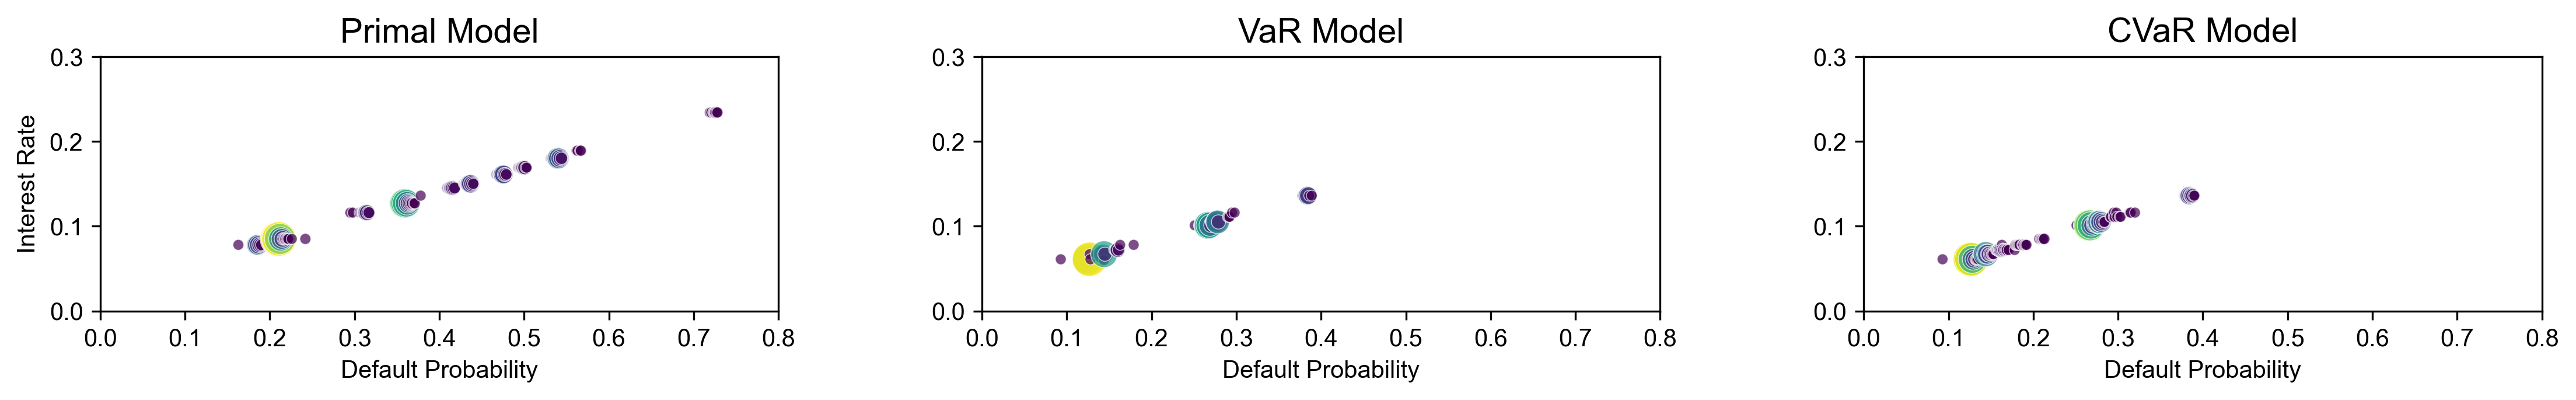
\includegraphics[width=\textwidth]{Figures/model_comparison_scatter.png}
\caption{三类模型下贷款样本在违约率与利率维度的联合分布}
\label{fig:combined_results}
\end{figure}

图~\ref{fig:boxplot_comparison} 从期望收益与贷款金额两个维度进一步分析了三类模型下贷款样本的特征分布。子图~\ref{fig:expected_profit_boxplot} 所示为期望收益的箱线图,揭示了各模型在收益集中趋势与离散程度方面的显著差异。其中,模型~\ref{eq:main_model} 拥有最高的收益中位数及最大波动性,表明其包含若干高收益高风险贷款;模型~\ref{eq:var_model} 的收益分布相对收敛,尾部波动被有效缓释;模型~\ref{eq:cvar_model} 在剔除极端高回报样本的基础上,呈现出更为集中的收益分布,进一步验证其稳健性。

子图~\ref{fig:loan_amount_boxplot} 展示了贷款金额的分布差异。结果显示,模型~\ref{eq:main_model} 与模型~\ref{eq:var_model} 倾向于选取大额贷款组合,尤其前者包含若干金额较高的样本;而模型~\ref{eq:cvar_model} 明显更偏好金额相对较小的贷款,以压缩潜在单笔损失规模,强化尾部风险的可控性。

\begin{figure}[htbp]
\centering
\subfigure[期望收益分布]{
  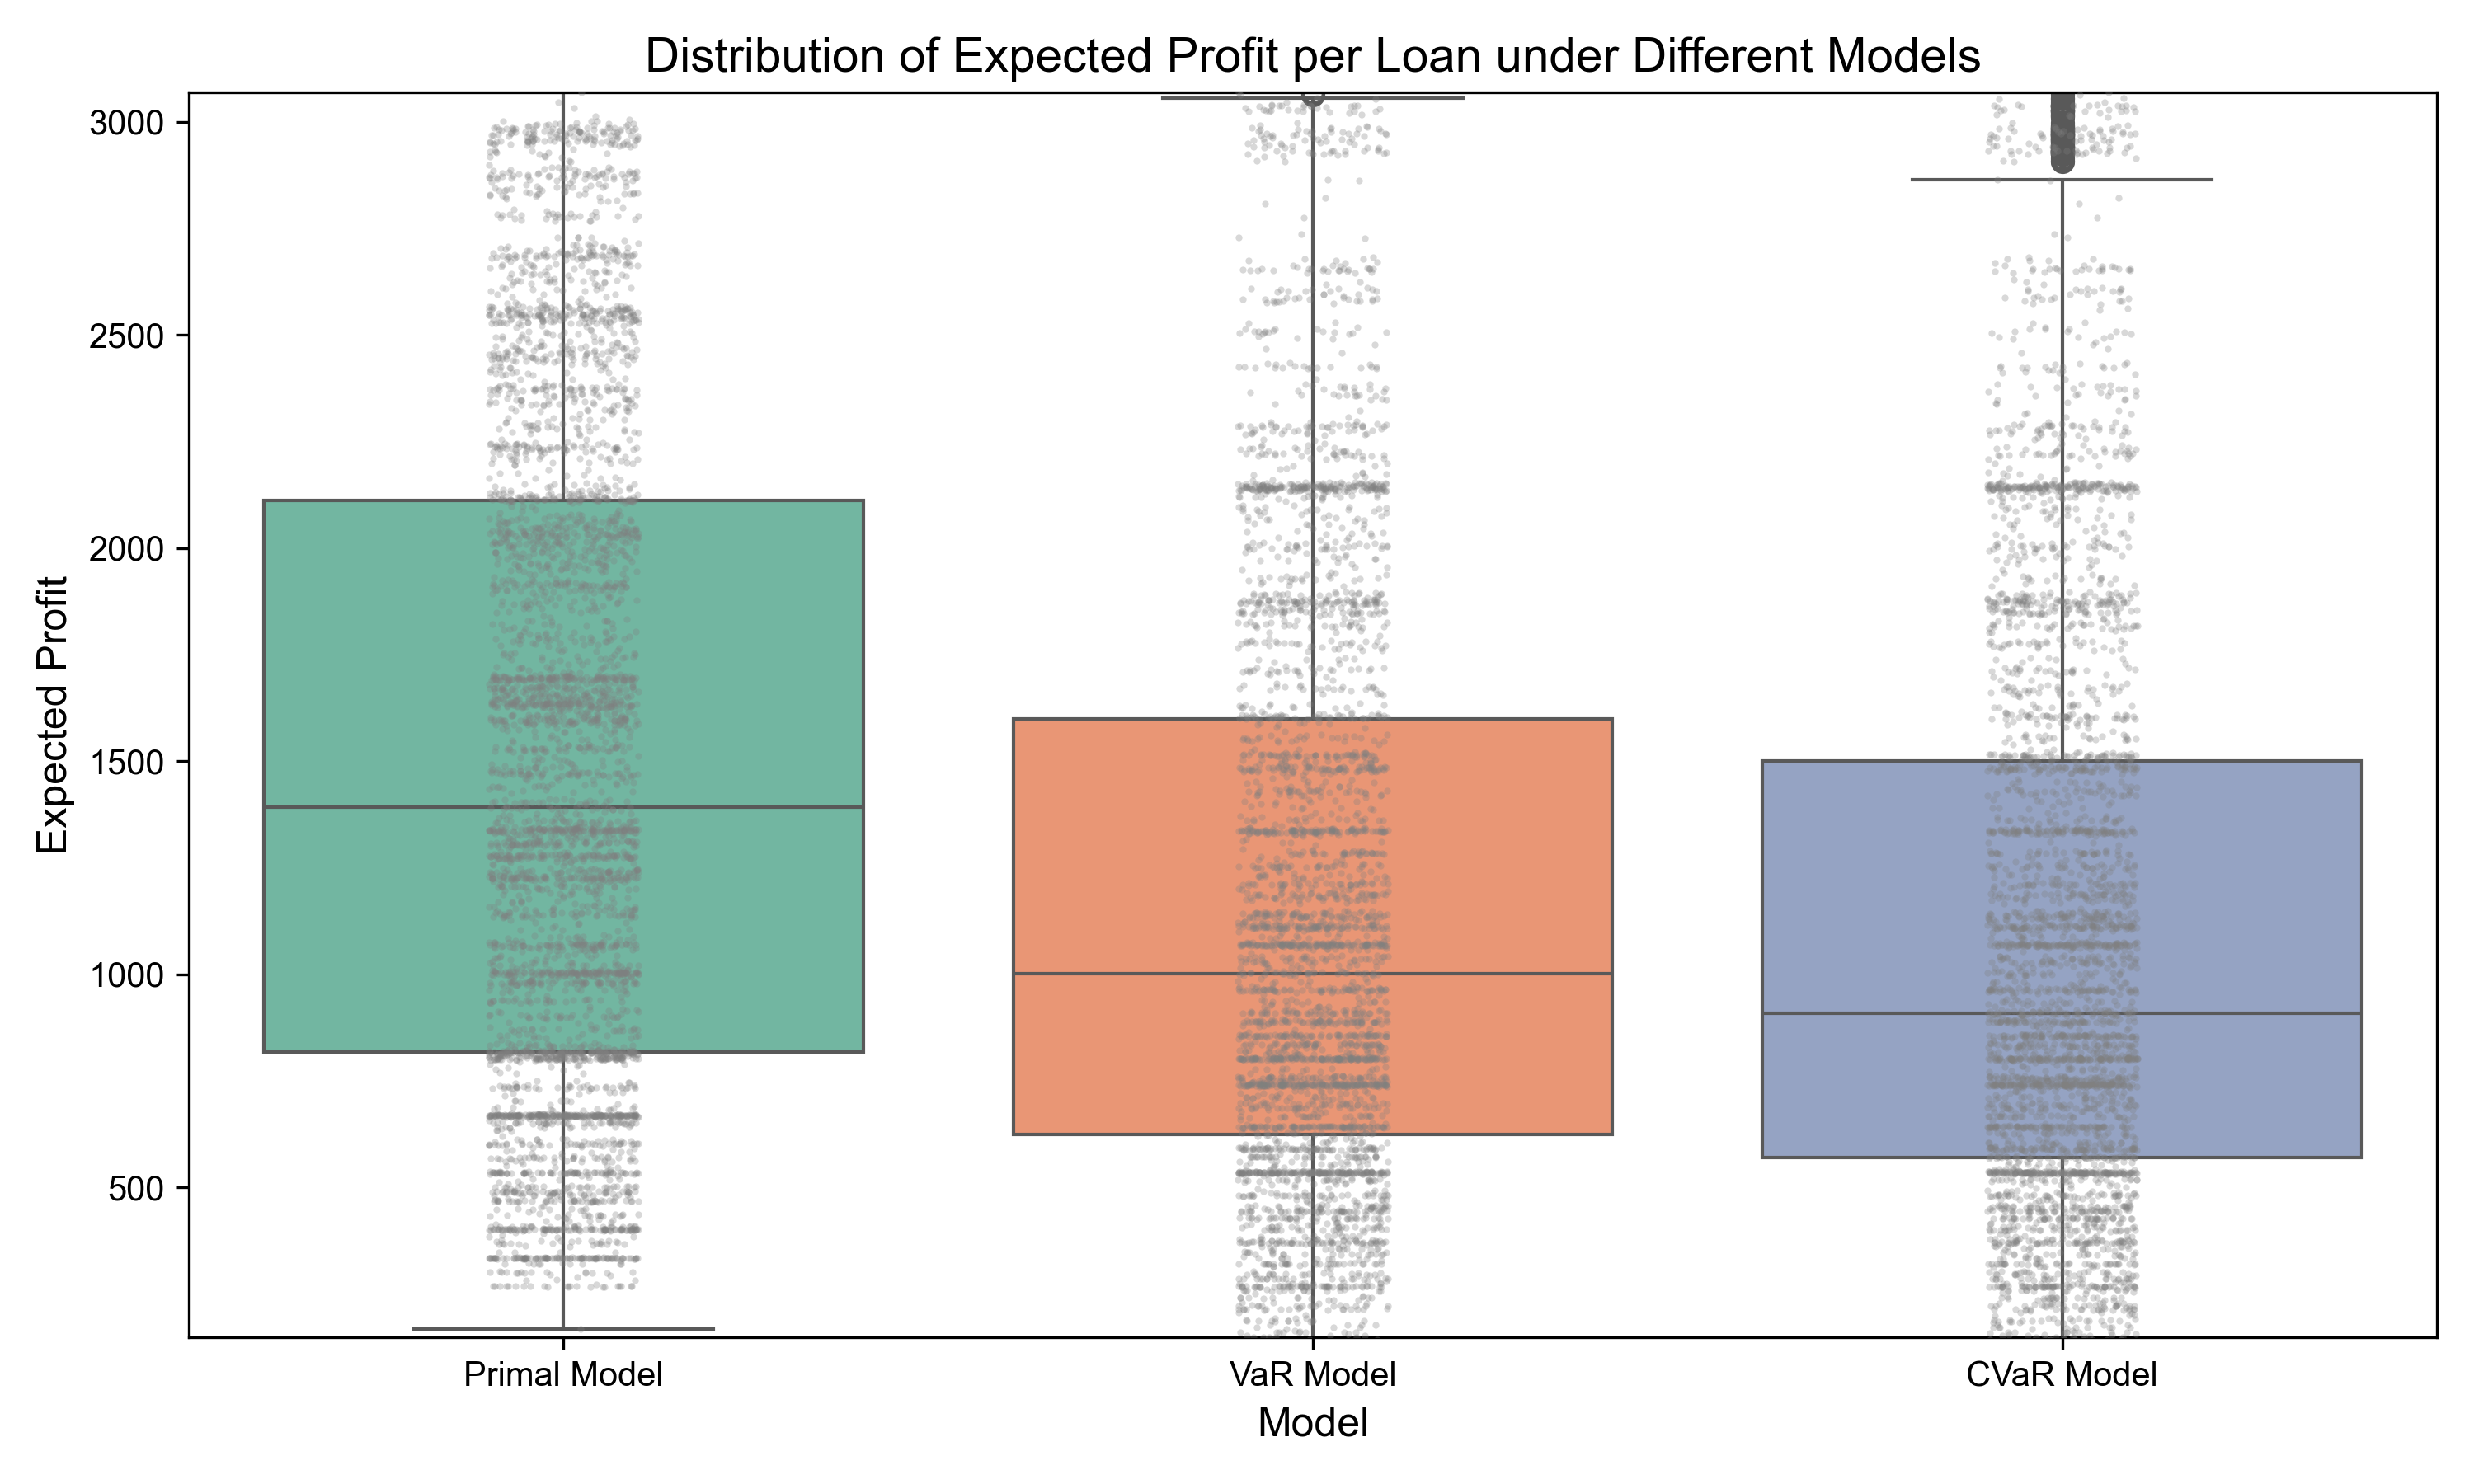
\includegraphics[width=0.48\textwidth]{Figures/model_comparison_expected_profit_boxplot.png}
  \label{fig:expected_profit_boxplot}
}
\subfigure[贷款金额分布]{
  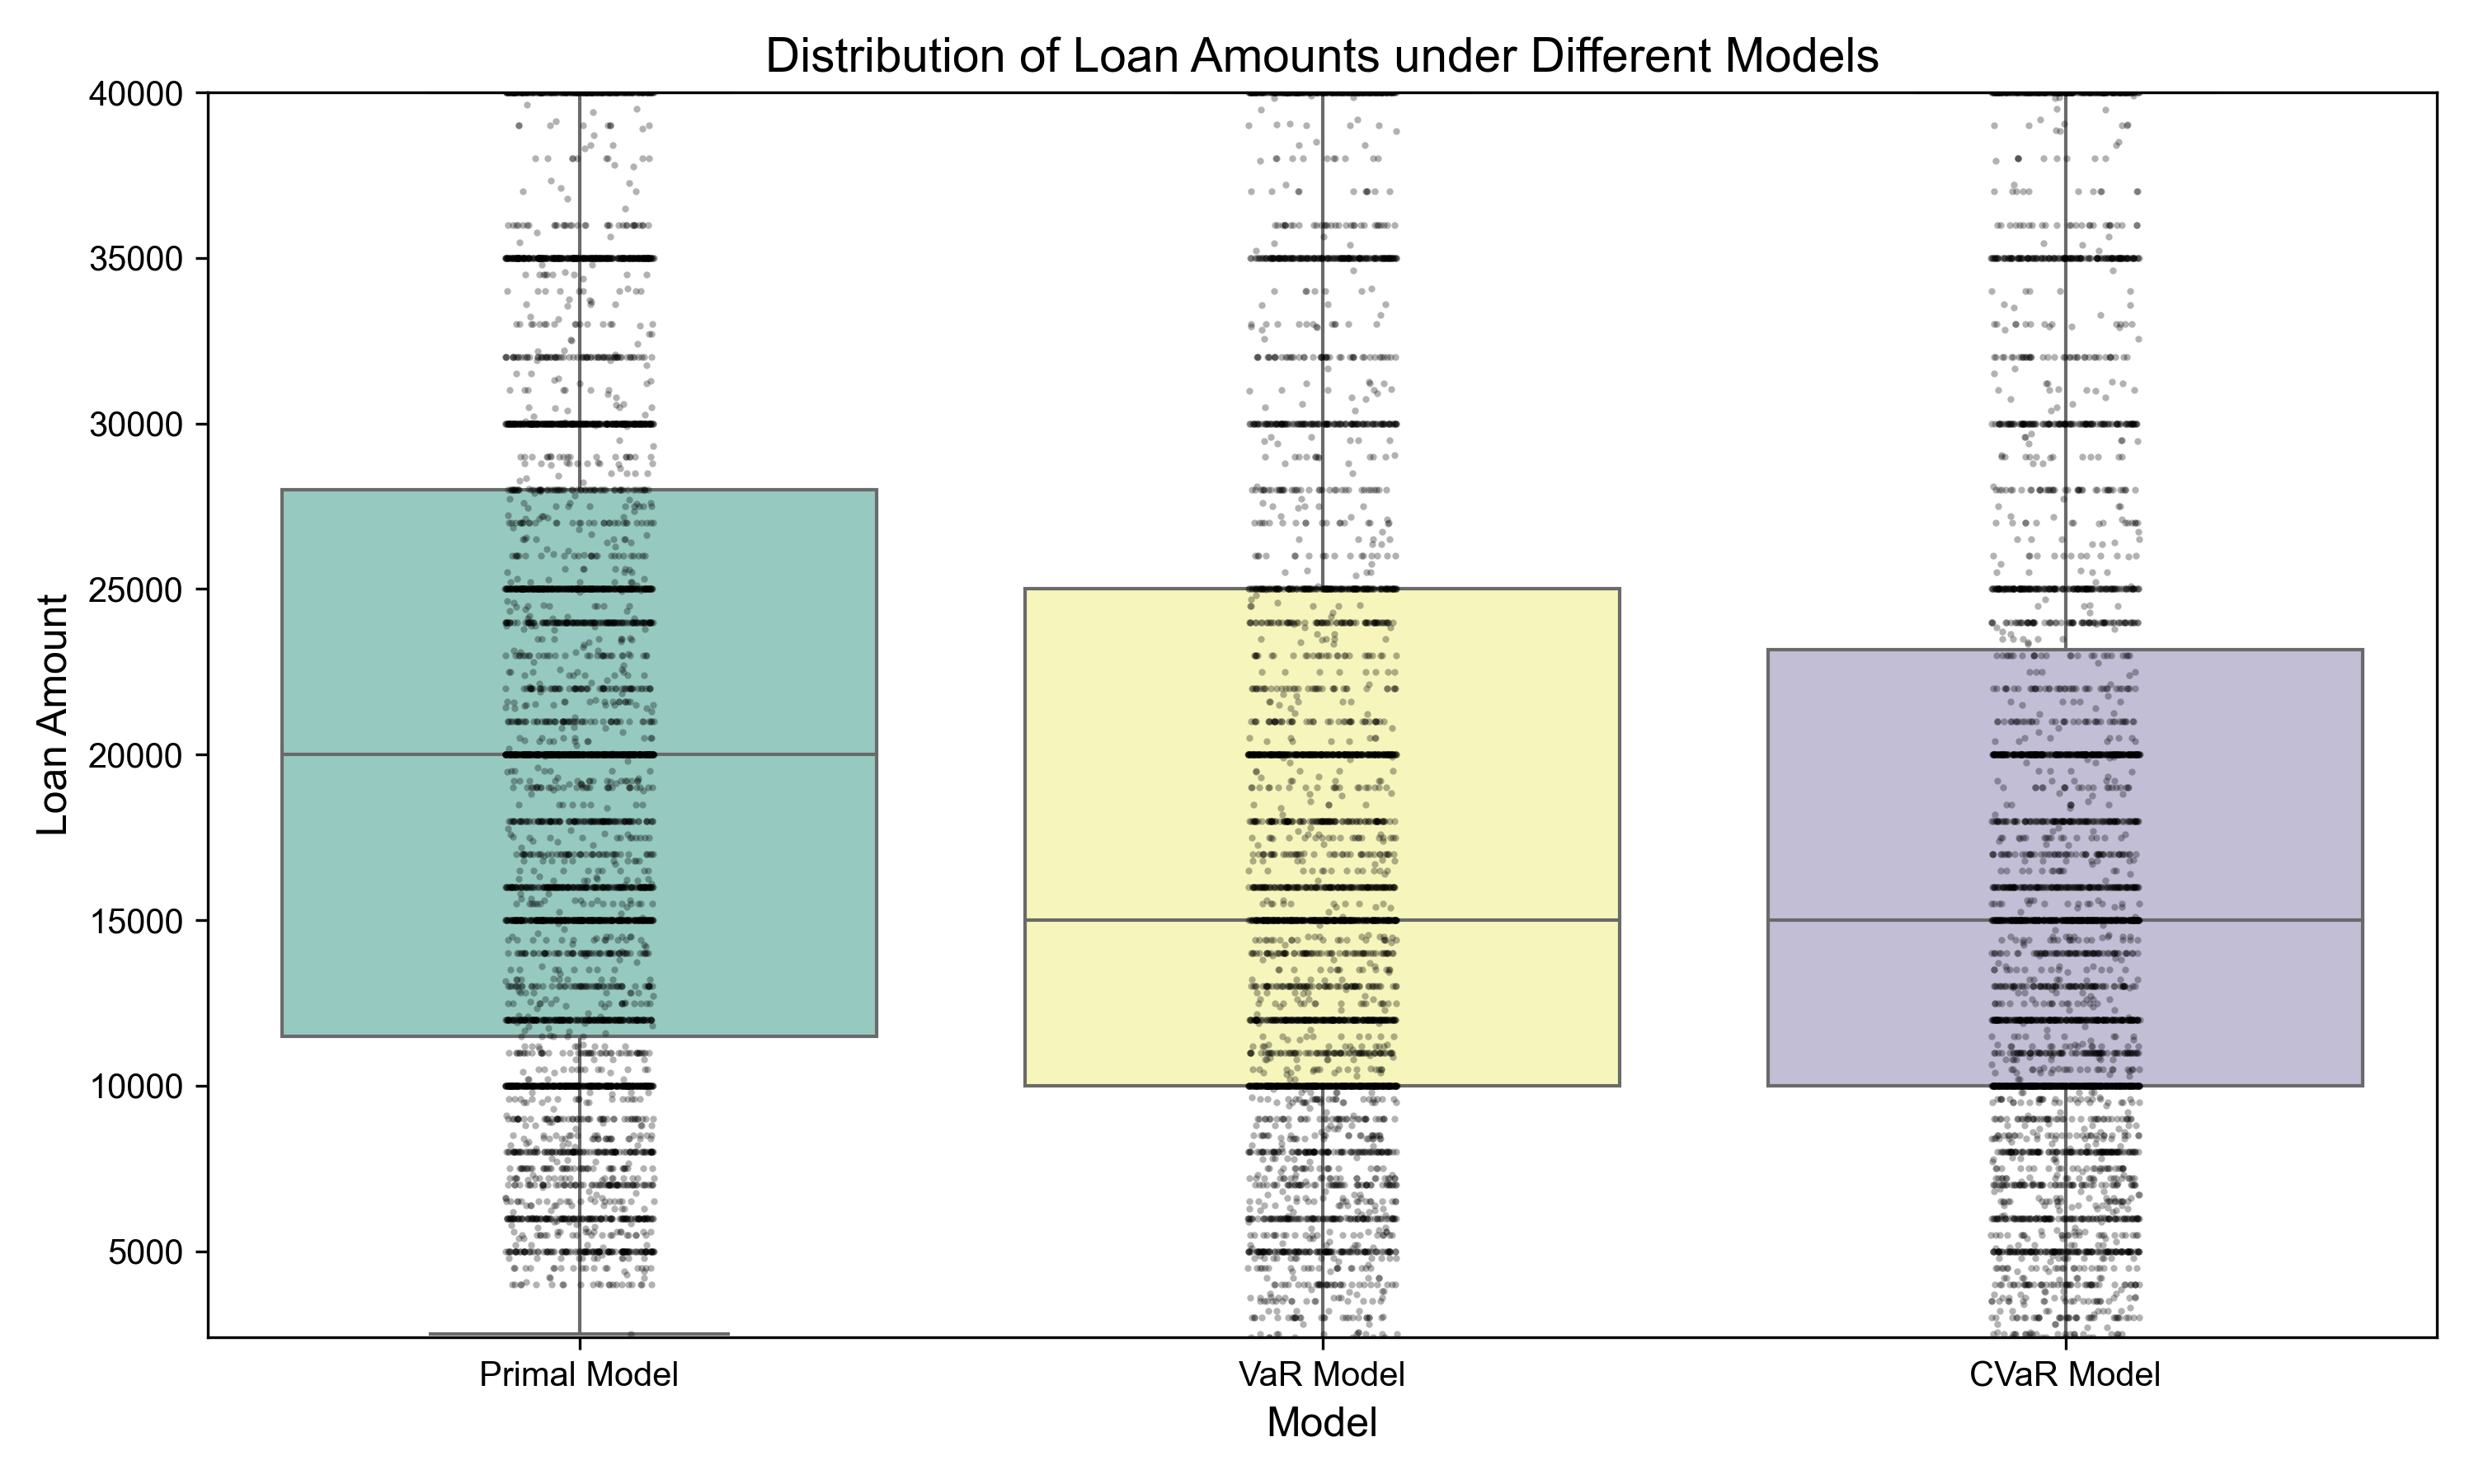
\includegraphics[width=0.48\textwidth]{Figures/model_comparison_loan_amount_boxplot.png}
  \label{fig:loan_amount_boxplot}
}
\caption{三类优化模型下的期望收益与贷款金额分布特征}
\label{fig:boxplot_comparison}
\end{figure}

综合来看,三类模型在贷款筛选机制、收益风险权衡策略与样本分布结构上均表现出高度异质性。模型~\ref{eq:main_model} 注重回报最大化,适用于风险容忍度较高的投资者;模型~\ref{eq:var_model} 在控制分位损失的基础上实现风险-收益平衡;模型~\ref{eq:cvar_model} 进一步强化尾部损失管理,体现出对极端风险的高度规避倾向。上述结果表明,在实际投资决策中,通过引入不同形式的风险约束不仅可以有效调整组合结构,也为多样化的投资者风险偏好提供了策略匹配的理论依据与实践工具,具有重要的现实意义与推广价值。
\section{结论与启示}
\label{sec:conclusion}

本文基于 Lending Club 平台的真实信贷数据,系统构建了三类贷款投资组合优化模型,分别为期望收益最大化模型、引入 VaR 约束的风险控制模型以及引入 CVaR 约束的稳健优化模型。模型综合考虑了投资预算限制、信用等级结构、贷款违约概率、极端损失发生概率与尾部损失均值等关键要素,能够灵活适配不同风险偏好的投资场景。为提升求解效率与解的质量,本文进一步设计了粒子群优化(PSO)与 Gurobi 联合优化框架,在保障计算可行性的同时,显著提升了解的精度与稳健性。

实证结果表明,不同模型在贷款组合选择策略、期望回报水平与尾部风险控制效果上存在显著差异。期望收益最大化模型在缺乏风险约束的条件下实现了最高的组合收益,但同时伴随着较高的尾部损失暴露;VaR 模型通过限制极端损失发生概率,在维持较高收益水平的同时实现了有效的风险控制;CVaR 模型则在牺牲部分期望回报的基础上,显著降低了尾部损失均值,体现出更强的稳健性与风险规避能力。上述结果表明,风险约束机制不仅显著改变了最优组合的结构特征,也对贷款筛选的风险收益权衡逻辑产生了实质性影响。

从平台管理与金融科技实践视角出发,本文的研究结论具有以下启示:(1)平台应推进风险控制模型的体系化建设,合理引入多维度风险约束(如 VaR、CVaR)以提升对极端违约事件的识别与应对能力;(2)风险容忍参数应结合用户画像与资金属性动态设定,实现收益与风险之间的自适应平衡;(3)模型生成的中间变量(如样本 CVaR、边际 VaR)可进一步用于贷后动态监测与风险预警,强化信贷业务的全过程风控闭环;(4)平台亦可基于模型输出构建分层次、差异化的智能投顾方案,满足投资者在多风险维度下的信贷资产配置需求。

从模型适用性的角度看,三类优化模型各具优势。期望收益最大化模型适用于风险承受能力强、追求高收益的投资者,尤其在宏观经济稳定或市场利率上行背景下表现良好;VaR 模型适合在兼顾监管合规与收益目标的中性风险场景中应用,如互联网银行的自动授信系统;而 CVaR 模型更适配于高稳健性场景,如养老金管理、保险资金配置或低风险资产池设计。三者构成了一个从“收益驱动”向“风险约束”递进的优化体系,为信贷资源的科学配置提供了可选择、可落地的建模架构。

需要指出的是,尽管我国 P2P 网络借贷平台已于 2020 年前后在政策引导下全面退出市场,但这并不削弱信贷组合优化问题的现实意义。目前,以消费金融公司、小额贷款公司、金融科技助贷平台等为代表的新型信贷主体,正在承接类似于 P2P 的资源配置功能。本文所提出的建模思想、优化框架与风险控制机制,依然适用于上述新型主体在产品设计、风险定价及智能投顾等应用场景中的实践需求。特别是在联合授信、额度动态调整、资金分层管理等新场景下,VaR/CVaR 风险指标可作为核心模块嵌入信贷决策流程,提升系统性风险防控能力。因此,尽管数据来源于美国市场,本文的方法论与结论对于我国金融科技行业在“后 P2P 时代”的信贷创新与监管转型仍具有较强的理论价值与应用推广意义。

综上所述,本文在建模层面实现了从目标函数设定、风险约束建构到算法求解策略的系统性设计;在实证层面揭示了不同风险控制机制对组合结构与绩效表现的具体影响;在应用层面提出了可迁移、可扩展的风险优化框架,服务于金融科技时代多元化主体的信贷资源配置需求。未来研究可进一步引入动态风险视角、多周期配置策略、投资者异质偏好刻画以及模型鲁棒性增强等方向,提升模型对复杂现实环境的适应力与解释力。


 
\section*{小组分工}%要出现在目录里面
\addcontentsline{toc}{section}{小组分工}
论文:张璐负责P2P模型建立和借贷背景调研,李晶晶负责违约概率预测,朱冯婧负责模型求解与结果分析。三人共同撰写论文内容。\\
PPT:张璐和李晶晶负责PPT的制作与展示。
 
\addcontentsline{toc}{section}{参考文献}
\bibliographystyle{gbt7714-2005-author-year}
\bibliography{ref}
%小组分工


\end{document}
